\section{Methods} \label{sec:methods}

\subsection{Equipment and preparations} \label{sec:methods:eq}

Figure \ref{fig:methods:equipment} shows all the equipment described in this section.

1. A \textbf{power supply} capable of providing $1000V$ or $30V$ DC.

2. A \textbf{parallel plate capacitor} with adjustable separation between the plates.

3. An \textbf{electrometer} capable of detecting small currents and measuring voltage in ranges, among others, $100V$, $10$ and $30V$. The range is selected with the FUNCTION knob. Besides, it must be discharged set the gauge needle set to $0V$ using the PUSH TO ZERO and/or ZERO LOCK knobs. The electrometer is grounded by connecting its $GND$ wire to the $GND$ pin of the power supply.

4. For grounding, the \textbf{grounding wrist bracelet} is used. It is grounded by connecting the bracelet wire to the $GND$ pin of the power supply.

5. The \textbf{Faraday cage}. It must be grounded by touching the inner and outer cage simultaneously with a grounded object (e.g., a hand with the wrist bracelet), and then releasing the inner cage and thereafter the outer cage.

6. A \textbf{black disk-on-a-rod}. It is further referred to as the rod.

7. A \textbf{conducting sphere} used as a charging station for the rod. It gains its electric potential by connecting it to the $1000V$ pin of the power supply.

\begin{figure}[H]
    \begin{subfigure}[b]{0.33\textwidth}
        \centering
        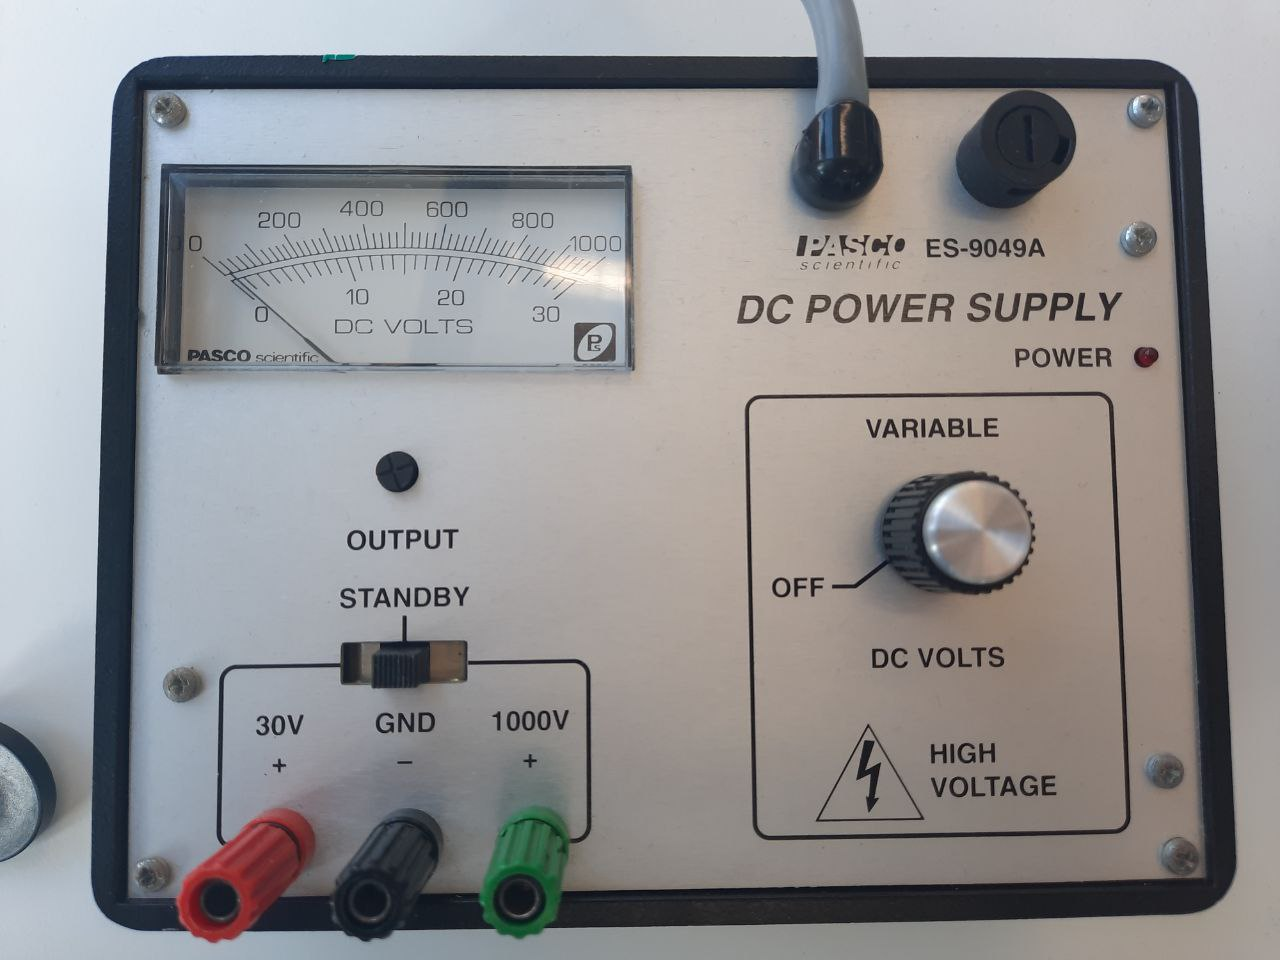
\includegraphics[width=\textwidth]{capacitors/img/setup/power_supply.jpg}
        \caption{Power supply}
    \end{subfigure}
    \begin{subfigure}[b]{0.33\textwidth}
        \centering
        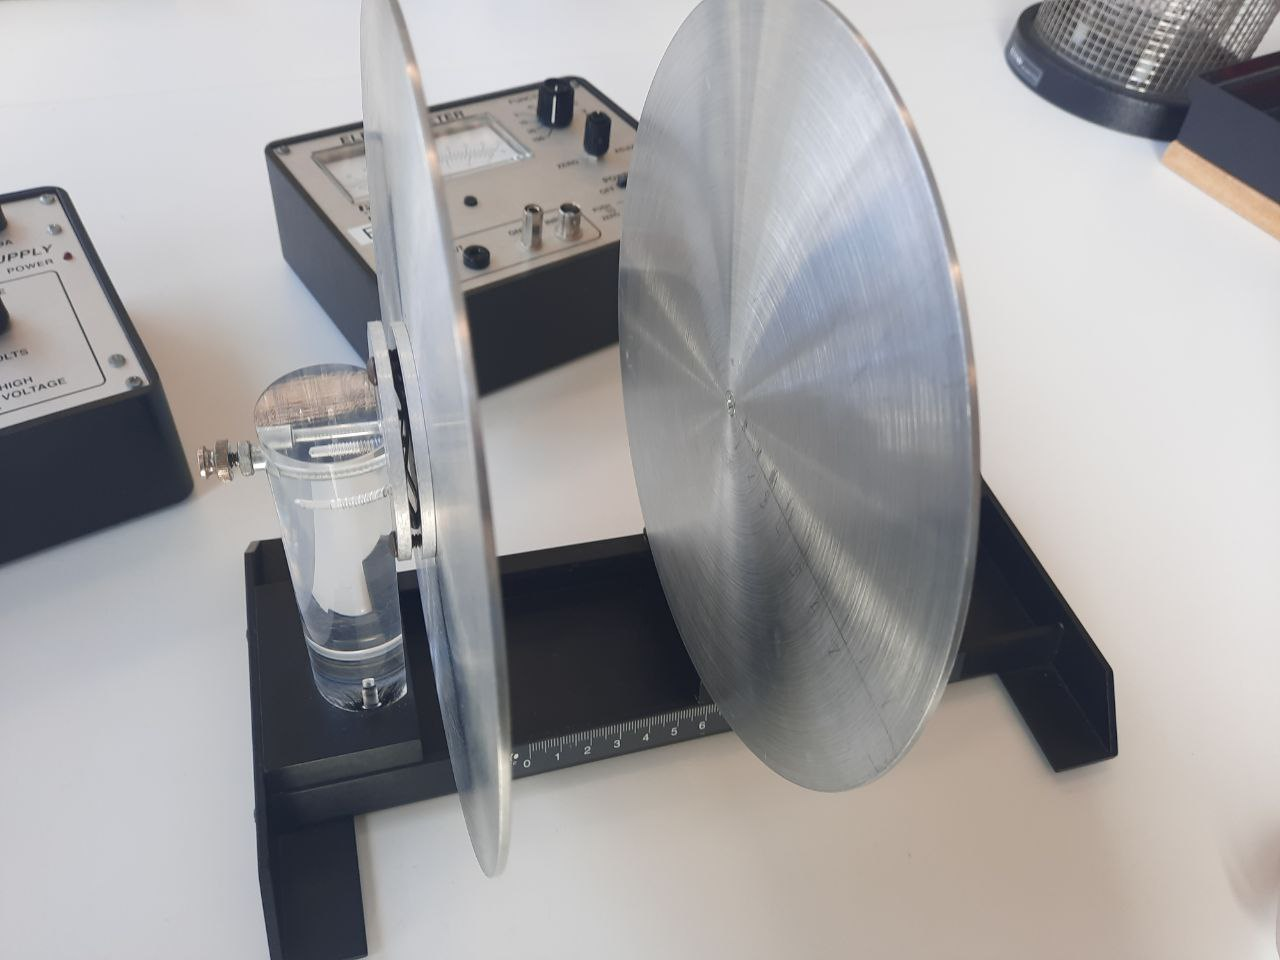
\includegraphics[width=\textwidth]{capacitors/img/setup/capacitor.jpg}
        \caption{Parallel-plate capacitor}
    \end{subfigure}
    \begin{subfigure}[b]{0.33\textwidth}
        \centering
        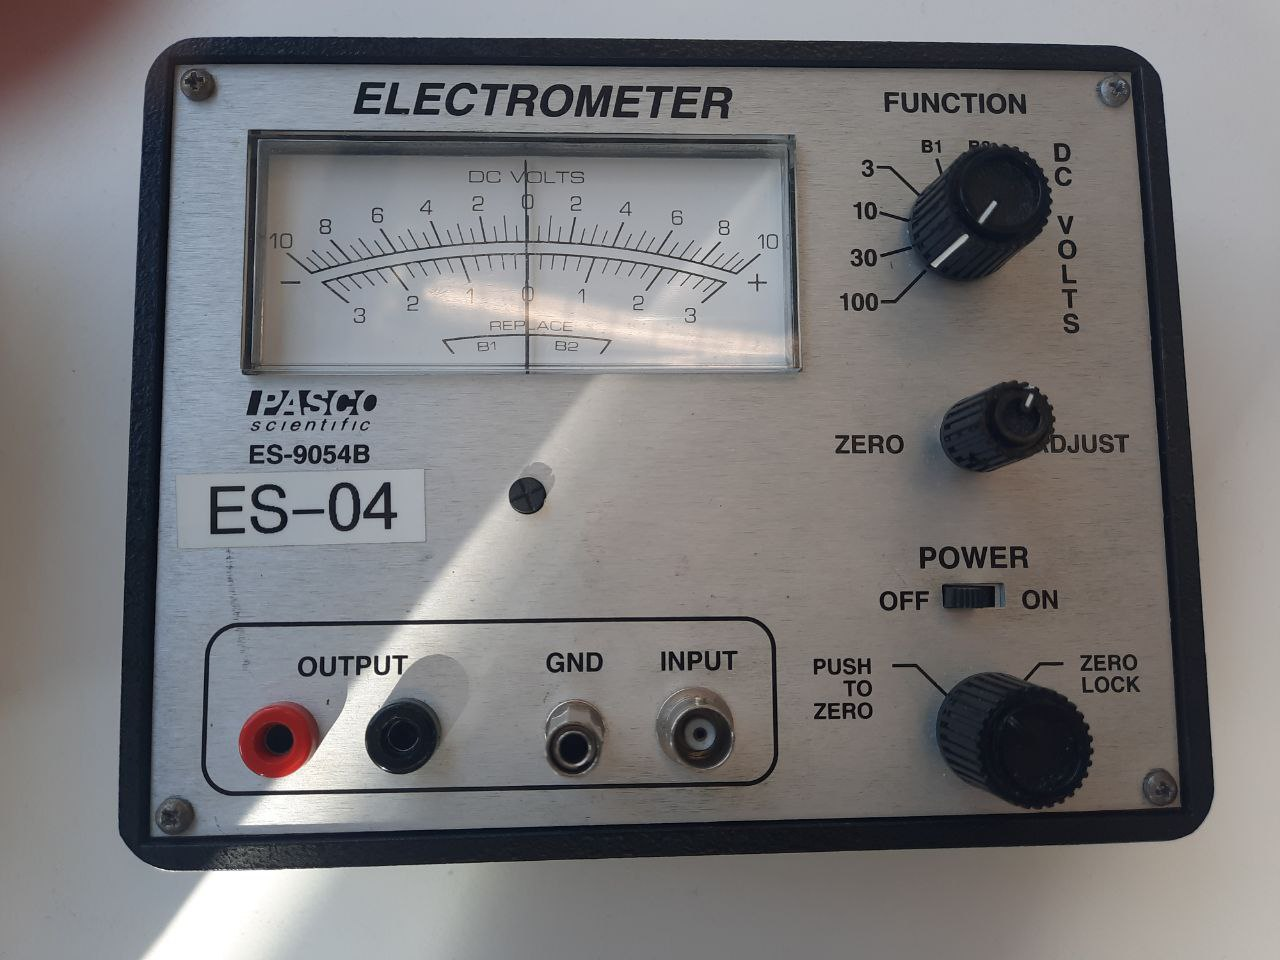
\includegraphics[width=\textwidth]{capacitors/img/setup/electrometer.jpg}
        \caption{Electrometer}
    \end{subfigure}
    
    \vspace{0.5cm}
    
    \begin{subfigure}[b]{0.33\textwidth}
        \centering
        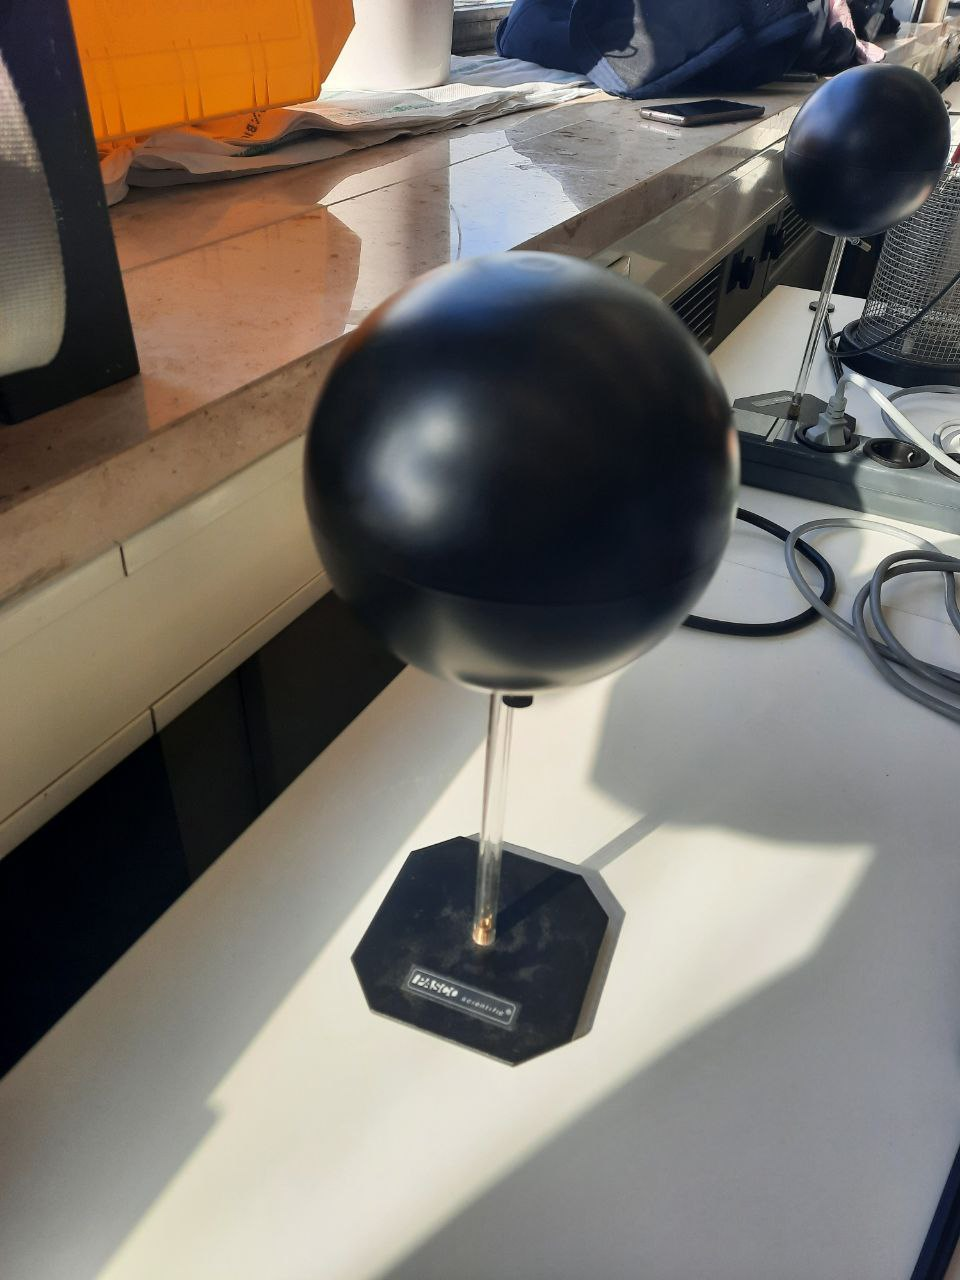
\includegraphics[width=\textwidth]{capacitors/img/setup/conducting_sphere.jpg}
        \caption{Conducting sphere}
    \end{subfigure}
    \begin{subfigure}[b]{0.33\textwidth}
        \centering
        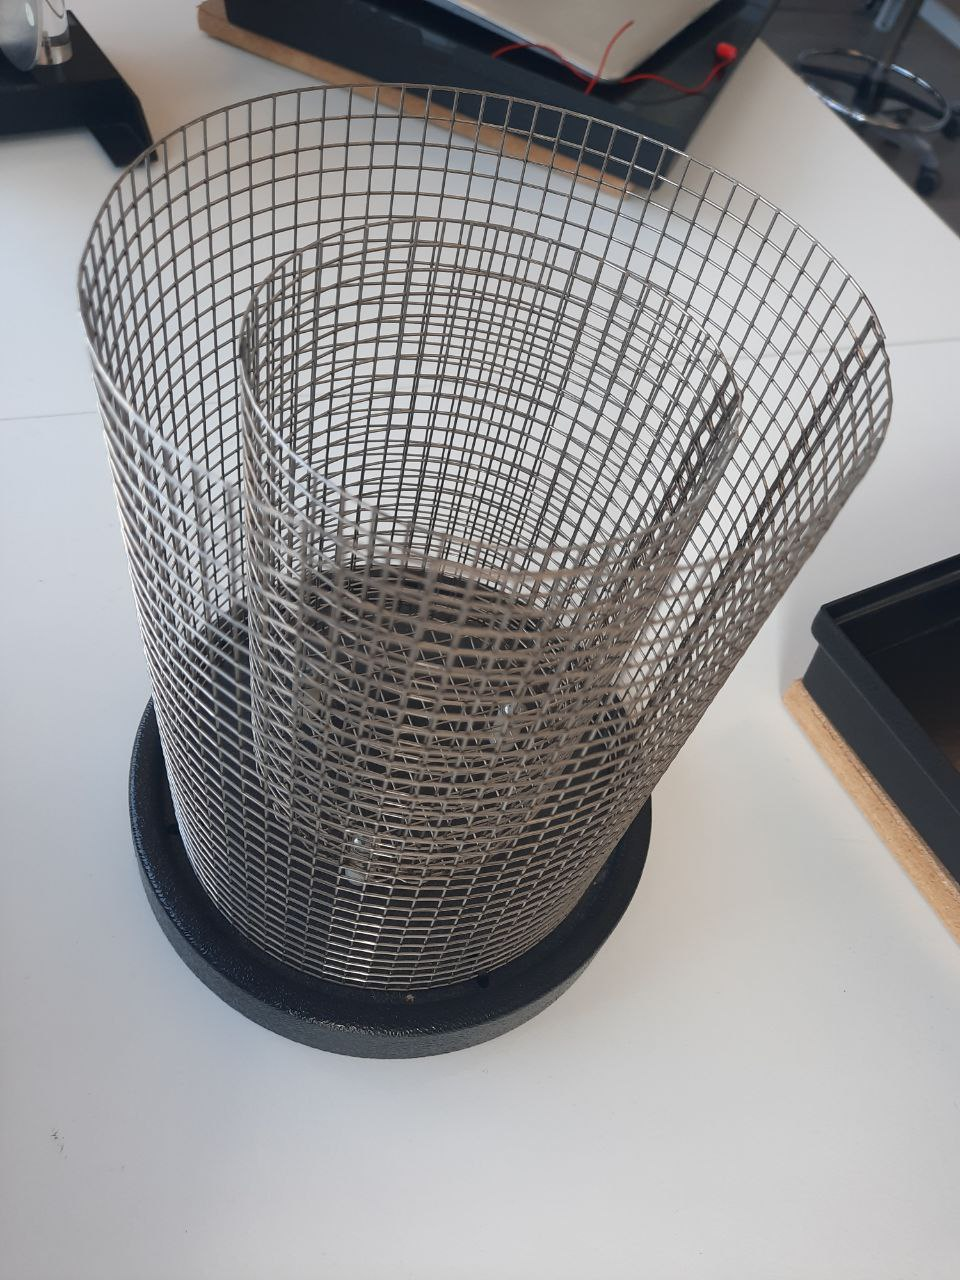
\includegraphics[width=\textwidth]{capacitors/img/setup/cage.jpg}
        \caption{Faraday cage}
    \end{subfigure}
    \begin{subfigure}[b]{0.33\textwidth}
        \centering
        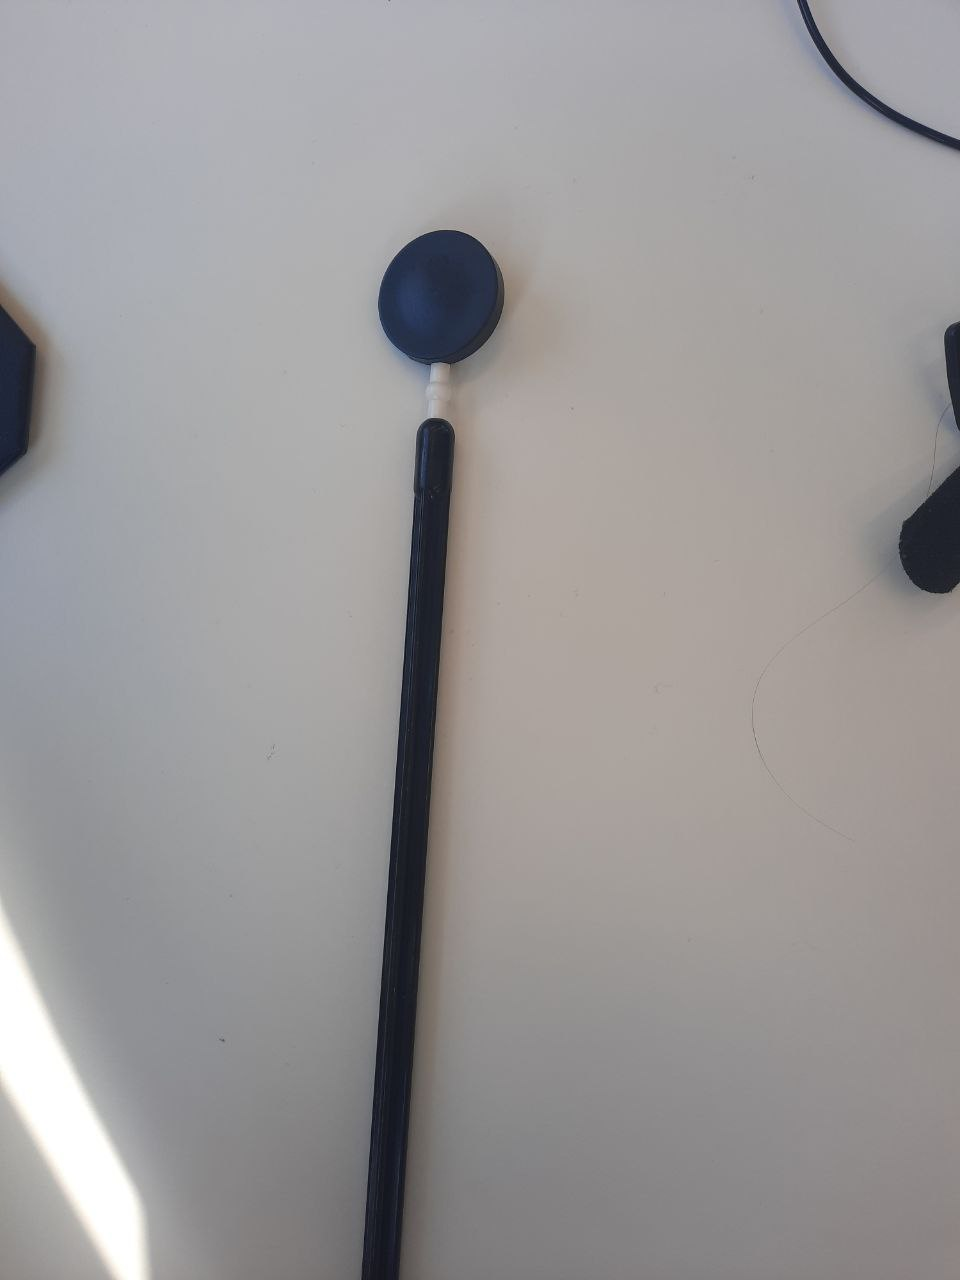
\includegraphics[width=\textwidth]{capacitors/img/setup/rod.jpg}
        \caption{Black disk-on-a-rod (the rod)}
    \end{subfigure}

    \vspace{0.5cm}

    \centering
    \begin{subfigure}[b]{0.33\textwidth}
        \centering
        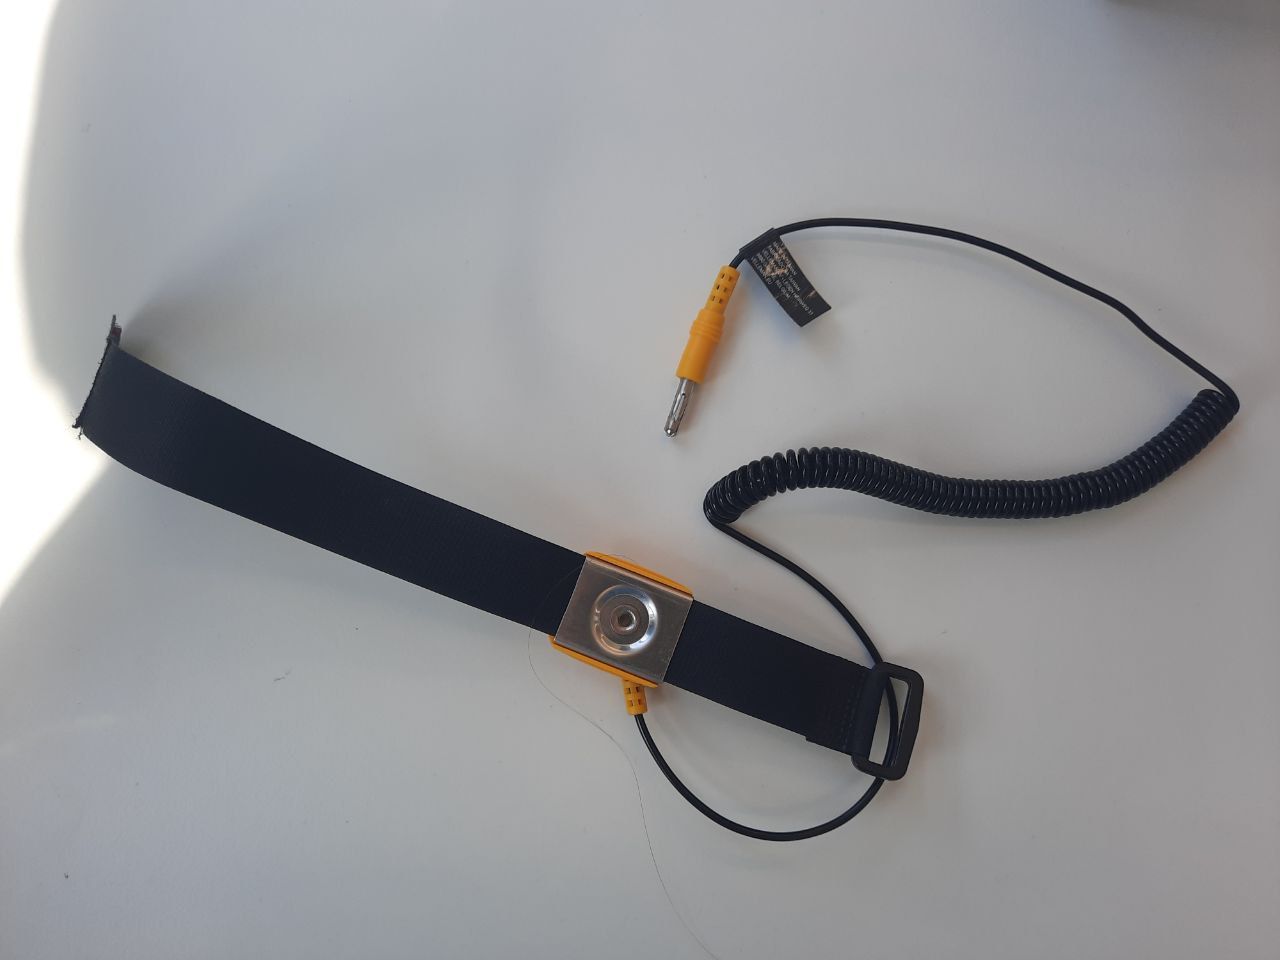
\includegraphics[width=\textwidth]{capacitors/img/setup/bracelet.jpg}
        \caption{Grounding wrist bracelet}
    \end{subfigure}
    
    \caption{Equipment}
    \label{fig:methods:equipment}
\end{figure}

\subsection{Part 1. The capacitor voltage as a function of charge} \label{sec:methods:exp1}

The separation of the capacitor is set to $s_{1} = 2 (mm)$. The conducting sphere is charged\footnote{The conducting sphere stays connected to the power supply.} to $1000V$ and placed at a distant from the capacitive circuit place. The capacitor is connected to the electrometer as shown in Figure \ref{methods:fig:capacitor_voltage}. The rod is touched to the sphere to gain some charge and then to the isolated (positive) plate of the capacitor to transfer this charge. The electrometer's measurement is noted. The table of the capacitor voltage as a function of the number of charges is made (10 measurements, 4 samplaes), and can be found in Table \ref{tab:appendix:data:exp1} in Appendix \ref{appendix:data}.  

\begin{figure}[H]
  \centering
  \includegraphics[width=0.5\textwidth]{capacitors/img/capacitor_voltage.png}
  \caption{The circuit for the finding the capacitor voltage as a function of charge}
  \label{methods:fig:capacitor_voltage}
\end{figure}

Then, the separation of the capacitor is set to $s_{2} = 4 (mm)$ and the same algorithm is conducted. Table \ref{tab:appendix:data:exp1} in Appendix \ref{appendix:data} contains tabular data for this separation as well.

Relation between the measured capacitor voltage and the number of charges applied is shown and discussed in Section \ref{sec:results:exp1}.

\subsection{Part 2. The distribution of charge on a surface} \label{sec:methods:exp2}

The capacitor is connected to the $1000 (V)$ pin of the power supply as shown in Figure \ref{methods:fig:distribution}. The electrometer is connected to the inner and outer cages of the Faraday cage. At each charge transfer, the Faraday cage and the rod are discharged. At each iteration, the rod is touched to the positive plate of the capacitor at some position $r$ from the center of the capacitor plate, and the charge of its vicinity will be transferred to the rod. Then, the rod is touched with the inner cage of the Faraday cage, leading to an emerging electric field from the inner cage which leads to some potential difference between the inner and outer cages. This voltage is used as a measure of charge at the position on the plate and is measured by the electrometer. This process is repeated at different positions along the radius of the capacitor plate ($11$ measurements, $3$ samples). Respective tabular data is located in Table \ref{tab:appendix:data:exp2} in Appendix \ref{appendix:data}.

\begin{figure}[H]
  \centering
  \includegraphics[width=0.5\textwidth]{capacitors/img/distribution.png}
  \caption{The circuit for the finding the surface charge distribution on the capacitor plate}
  \label{methods:fig:distribution}
\end{figure}

The \textit{surface charge density} is obtained from the voltage-position graph, and is shown and discussed in Section \ref{sec:results:exp2}.

\subsection{Part 3. The potential difference as function of the plate distance at constant charge} \label{sec:methods:exp3}

The capacitor plate separation is initially set to $s_{1} = 2 (mm)$. The capacitor is charged with the $20V$ output from the power supply, and this charge remains stored in the capacitor after disconnecting the power supply. The electrometer's range is set to $100V$. The capacitor voltage is measured for different capacitor plate separations from $s_{1} = 2 (mm)$ up to the maximum distance possible $s_{max} = 12 (cm)$ (in total $13$ measurements, $5$ samples). The obtained data is located in Table \ref{tab:appendix:data:exp3} in Appendix \ref{appendix:data}.
